\begin{figure}[htbp]
  \centering

  \begin{subfigure}[t]{0.48\textwidth}
    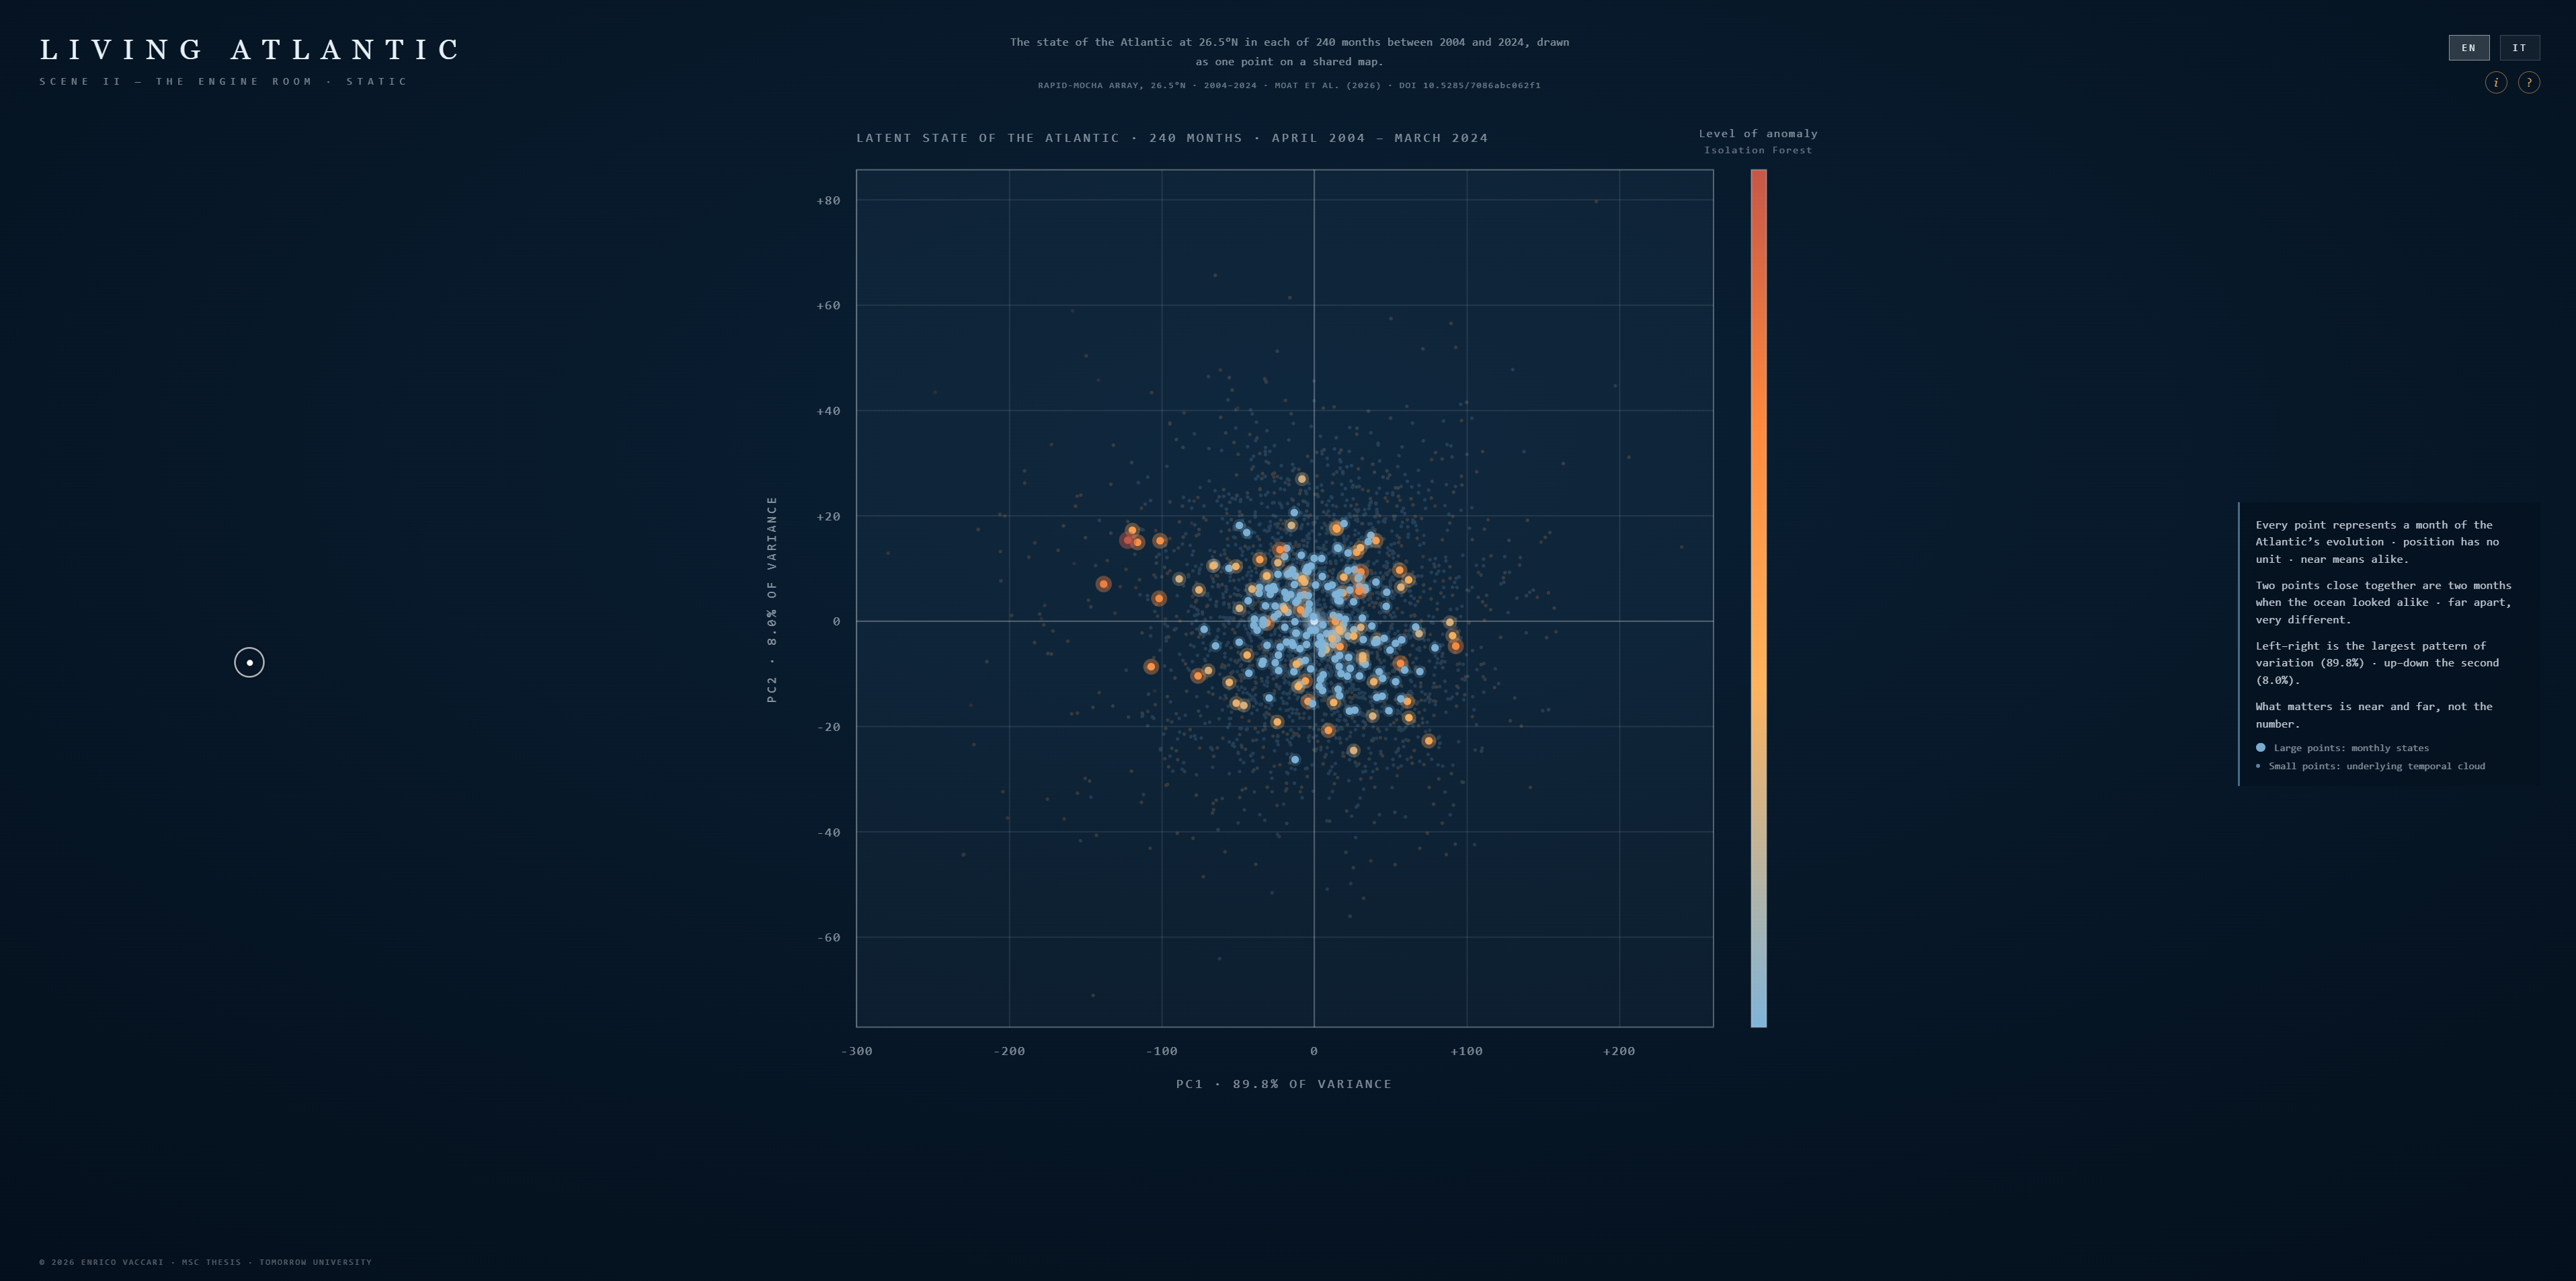
\includegraphics[width=\textwidth]{figures/viz2/viz2_theengine-static.png}
    \caption{Controllo (C1): la rappresentazione statica dello spazio latente.}
    \label{fig:theengine-static}
  \end{subfigure}
  \hfill
  \begin{subfigure}[t]{0.48\textwidth}
    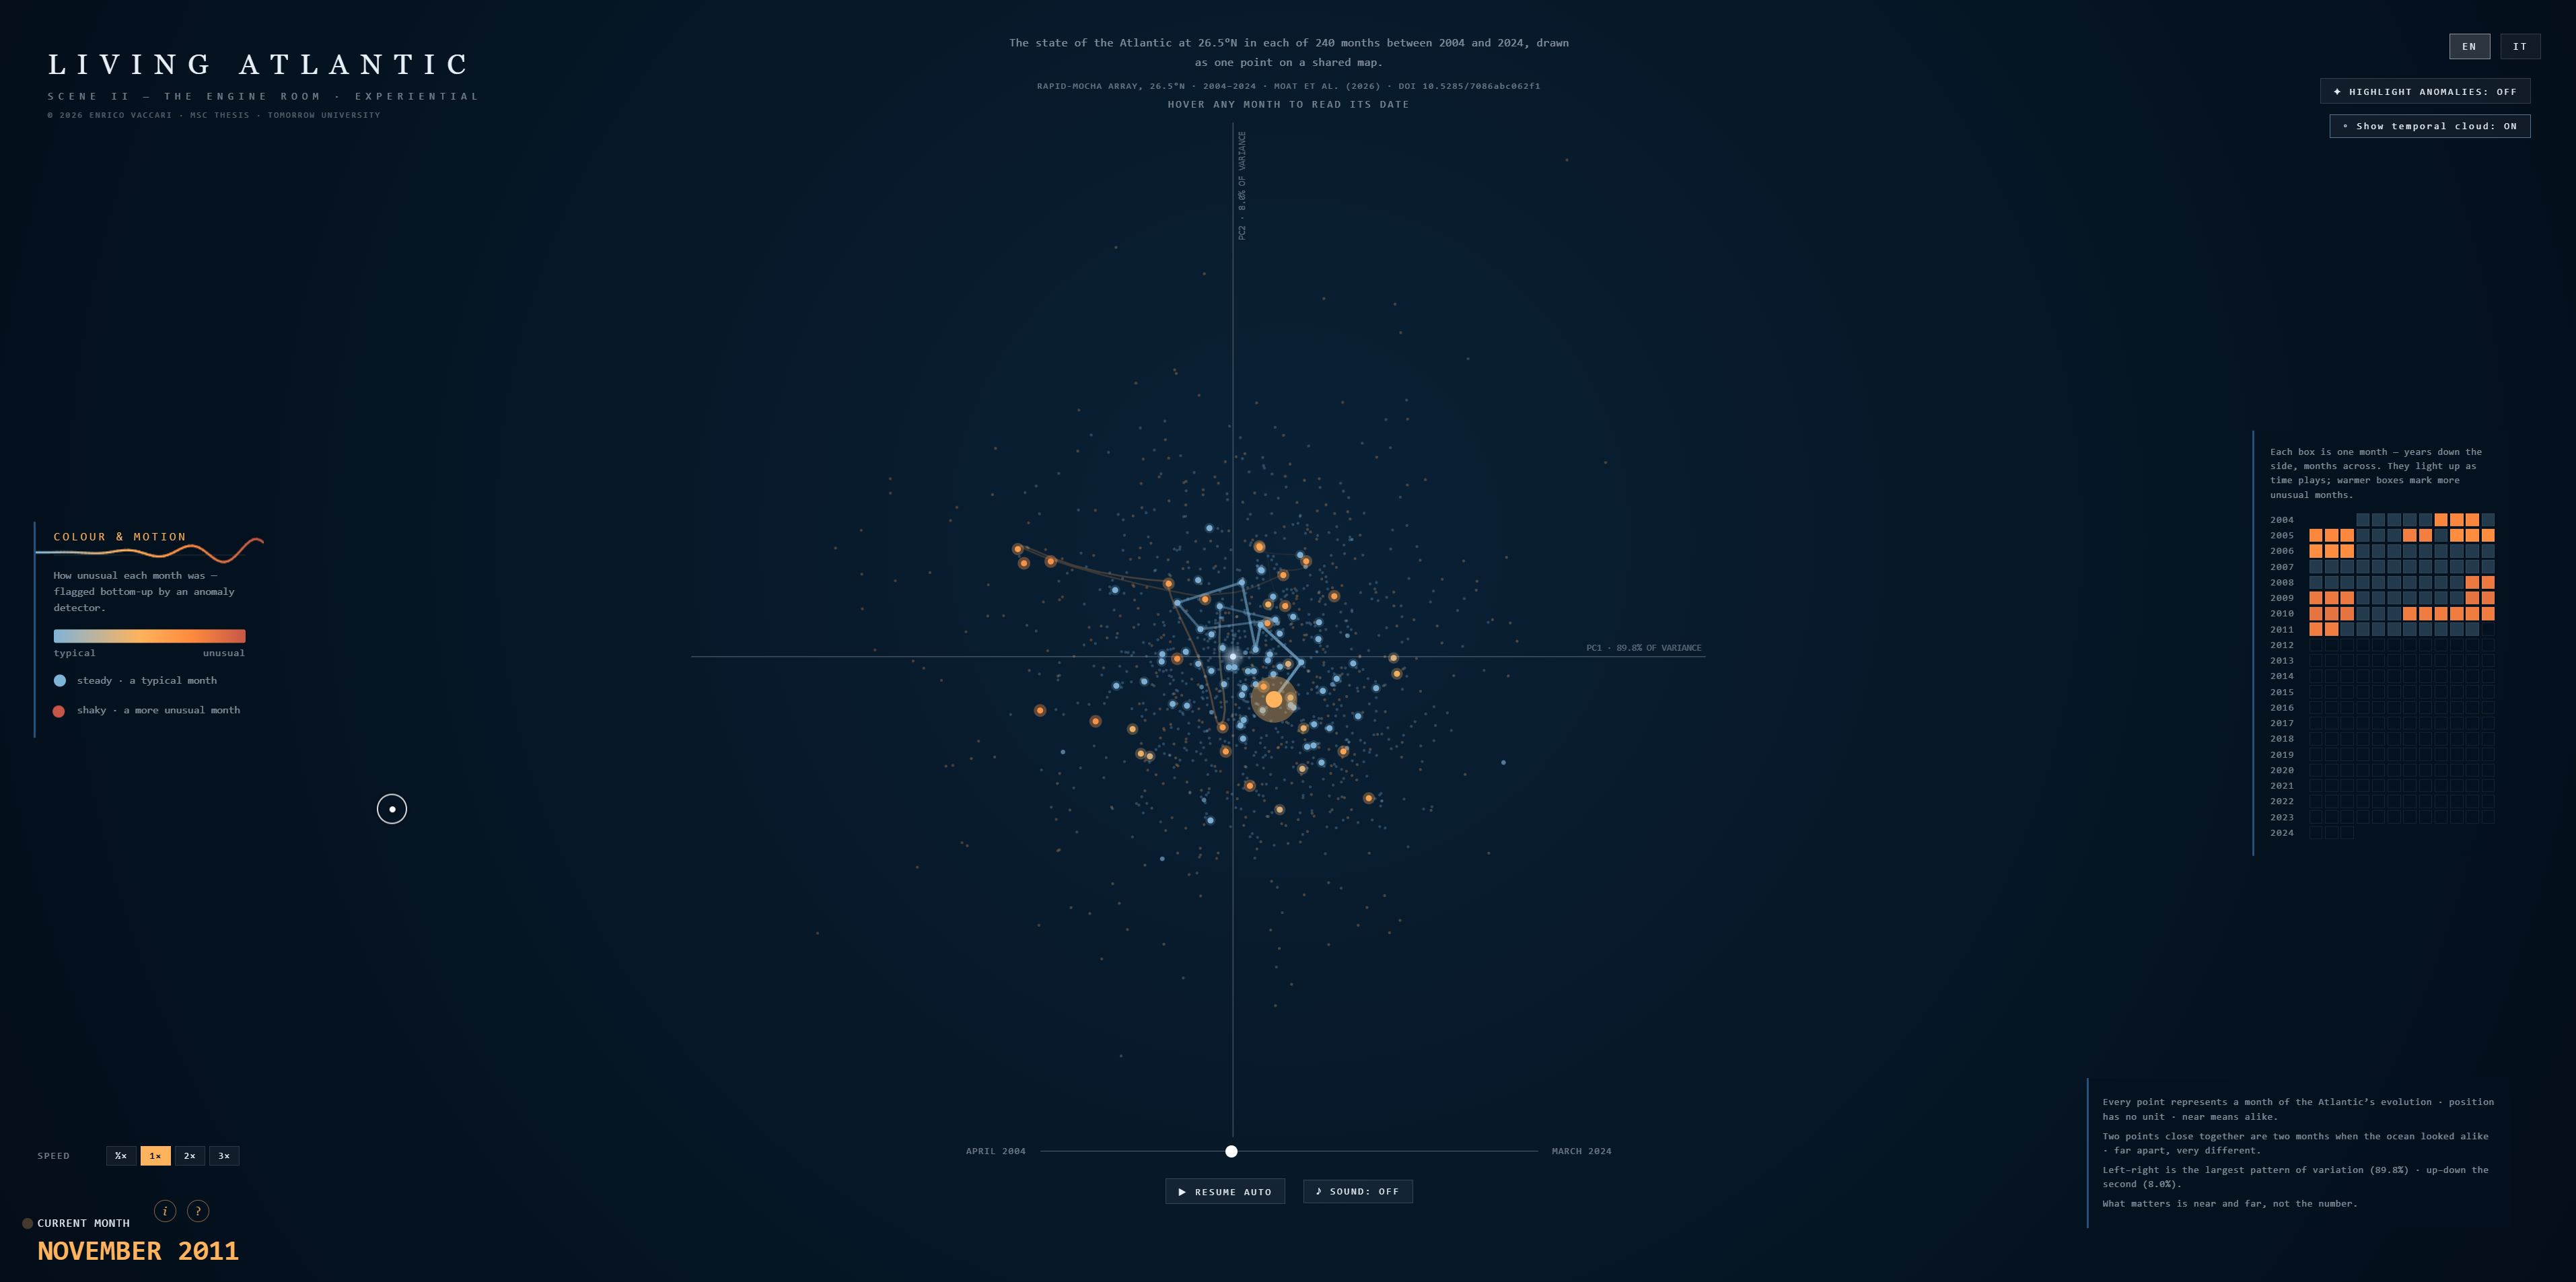
\includegraphics[width=\textwidth]{figures/viz2/viz2_theengine-experiential.png}
    \caption{Esperienziale (C2+C3): la traiettoria in evoluzione attraverso lo spazio latente.}
    \label{fig:theengine-experiential}
  \end{subfigure}

  \caption[Le due condizioni della Scena~II]{Le due condizioni somministrate della
  Scena~II, tratte dalle stesse coordinate latenti nel bundle di dati. La condizione
  statica mostra gli stati mensili come uno scatter fisso; la condizione esperienziale
  percorre gli stessi stati nel tempo.}

  \label{fig:theengine-conditions}
\end{figure}
